% main_report64.tex
% SAMBP TR-64/2026 -- IBR-Aware 87T Integration: SPRT + Zone Model
% Compile: pdflatex -> bibtex -> pdflatex -> pdflatex
\documentclass[11pt, a4paper]{article}

\usepackage[T1]{fontenc}
\usepackage[utf8]{inputenc}
\usepackage[margin=25mm]{geometry}
\usepackage{amsmath, amssymb, amsthm}
\usepackage{booktabs, array, multirow}
\usepackage{graphicx}
\usepackage{xcolor}
\usepackage{hyperref}
\usepackage{pgfplots}
\pgfplotsset{compat=1.18}
\usepackage{tikz}
\usetikzlibrary{arrows.meta, positioning, calc, fit, backgrounds, shapes.geometric}
\usepackage{caption}
\usepackage{subcaption}
\usepackage{parskip}
\usepackage{natbib}
\usepackage{pifont}
\usepackage{listings}
\usepackage{algorithm}
\usepackage{algpseudocode}

\hypersetup{colorlinks=true, linkcolor=blue!60!black, citecolor=blue!60!black,
            urlcolor=blue!60!black}

\definecolor{okgreen}{RGB}{0,130,60}
\definecolor{alertred}{RGB}{180,0,0}
\definecolor{ibrbrown}{RGB}{130,60,0}

\newtheorem{proposition}{Proposition}
\newtheorem{lemma}{Lemma}
\newtheorem{corollary}{Corollary}
\newtheorem{remark}{Remark}

\newcommand{\pu}{\,\text{pu}}
\newcommand{\ms}{\,\text{ms}}
\newcommand{\Hz}{\,\text{Hz}}
\newcommand{\kn}{\kappa_n}
\newcommand{\fint}{f_{\rm int}}
\newcommand{\kibr}{k_{\rm ibr}}
\newcommand{\Ak}{A_k}

\title{\textbf{SAMBP TR-64/2026}\\[4pt]
       \large IBR-Aware Transformer Differential Protection:\\
       Integration of Three-Hypothesis SPRT with Zone Model (87T)}
\author{PhD Candidate\\[2pt]
        \small Smart Adaptive Multi-Bus Protection Research}
\date{April 2026}

% ============================================================================
\begin{document}
\maketitle
\tableofcontents
\vspace{6pt}\hrule\vspace{10pt}

% ============================================================================
\section{Background and Motivation}
\label{sec:background}

\subsection{Conventional 87T and the 2nd-Harmonic Blocking Mechanism}

The percentage-differential relay (87T) operates when the operate current
$I_{\rm op} = |I_H + I_X|$ exceeds the restraint characteristic.  To prevent
false tripping during transformer energisation (inrush), relay manufacturers
introduced 2nd-harmonic blocking in the 1950s~\cite{Kennedy1950}:

\begin{equation}
  \text{Block if}\quad
  \frac{I_{2f}}{I_{1f}} > H_{2,\rm thresh} \quad (= 0.15\text{ typically}).
  \label{eq:h2block}
\end{equation}

The physical basis of this rule is sound for synchronous-generator (SG)
networks: inrush current is rich in 2nd harmonic ($I_{2f}/I_{1f} \approx
0.3$--$0.9$), while SG fault current — driven by an AC source — has
$I_{2f}/I_{1f} < 0.05$.

\subsection{The IBR Gap}
\label{sec:ibr_gap}

IBR fault current is produced by the inverter's current controller, which
enforces a sinusoidal output with prescribed amplitude.  The SRF (synchronous
reference frame) current controller drives the DC component to zero within
one control period~\cite{Rocabert2012}.  However, the transformer core
introduces a residual-flux (remanence) contribution $B_r$ to the differential
current at fault inception:

\begin{equation}
  i_{\rm diff}(t) = (1-\kibr)\,i_{\rm SG}(t) + \kibr\,i_{\rm IBR}(t)
                    + B_r\,I_{\rm pk}\,e^{-t/\tau_r}\sin(2\omega t),
  \label{eq:idiff_ibr}
\end{equation}
where $\tau_r = 50\,\ms$ is the core-remanence decay time constant and
$B_r \in [0, 1]$ quantifies the per-unit residual flux.

For $\kibr \geq 0.7$ (IBR-dominated fault) with $B_r > 0$:
\begin{itemize}
  \item The IBR AC current has no DC offset; the Br term injects 2nd harmonic
    into the first 2--3 cycles.
  \item $I_{2f}/I_{1f}$ exceeds $H_{2,\rm thresh} = 0.15$ in the first cycle
    → 2nd-harmonic blocking fires → conventional 87T \textbf{RESTRAINS}.
  \item The protection \emph{misses the fault}: a false negative.
\end{itemize}

This is the \textbf{IBR gap} that TR-64 closes.  At $\kibr = 1.0$,
$B_r \in [0, 0.7]$, the conventional relay achieves only
$P_D^{\rm conv} = 0.24$, meaning \textbf{76\% of IBR-dominated internal
faults go undetected}.

\subsection{Scope and Relation to Prior TRs}

\begin{itemize}
  \item \textbf{TR-57} \cite{SAMBP_TR57} designed and validated the
    three-hypothesis SPRT for the 87T problem.  TR-64 imports its SPRT
    engine (Algorithm~1) and waveform generators directly.
  \item \textbf{TR-57a/b/c} validated SPRT to $P_D = P_{D2} = 1.000$,
    $P_{\rm FA} < 0.001$ on 24 deterministic scenarios and 30\,k MC trials.
  \item \textbf{TR-64} (this document) integrates the SPRT with the existing
    zone model to produce a unified IBR-aware relay that closes the IBR gap.
    It contributes to Chapter~5 (\emph{Transformer Differential 87T})
    alongside TR-57.
\end{itemize}


% ============================================================================
\section{Why SPRT Resolves the IBR Gap}
\label{sec:sprt_ibr}

\subsection{The Waveform Asymmetry Index}

The SPRT operates on the per-cycle waveform asymmetry index \cite{SAMBP_TR57}:
\begin{equation}
  \Ak = \frac{I_k^+ - |I_k^-|}{I_k^+ + |I_k^-|},
\end{equation}
where $I_k^+$ and $I_k^-$ are the positive and negative peak currents in
cycle $k$.

\begin{itemize}
  \item \textbf{Inrush (H0):} magnetising core current flows in one polarity
    only → $\Ak \approx +0.70$.
  \item \textbf{IBR internal fault (H1):} SRF controller maintains symmetric
    current → $\Ak \approx 0$, regardless of $\kibr$ or $B_r$.
  \item \textbf{External fault + CT saturation (H2):} CT recovery pulse
    creates asymmetric differential → $\Ak \approx -0.50$.
\end{itemize}

The key property for TR-64: $\Ak$ is \textbf{IBR-insensitive}.  Adding more
IBR (increasing $\kibr$) moves $\Ak$ toward 0 (more symmetric), which
strengthens the H1 classification, not weakens it.  The 2nd-harmonic Br
injection does \emph{not} affect $\Ak$ because it adds equal energy to both
half-cycles.

\subsection{SPRT Decision Boundaries}

The dual SPRT from TR-57 uses Wald boundaries $\pm B = \pm 6.91$ nats
($\alpha = \beta = 0.001$):
\begin{align}
  S_n &= \textstyle\sum_k \log\frac{f_{H1}(\Ak)}{f_{H0}(\Ak)}
         \quad \text{TRIP at } S_n \geq +B, \\
  S_n^{(2)} &= \textstyle\sum_k \log\frac{f_{H2}(\Ak)}{f_{H1}(\Ak)}
         \quad \text{CTALARM at } S_n^{(2)} \geq +B.
\end{align}
For a pure IBR fault ($\Ak = 0$ every cycle), each LLR increment $\lambda_k
= \log[f_{H1}(0)/f_{H0}(0)] \approx +3.4$\,nats (large positive), so the
boundary is crossed in at most $\lceil 6.91/3.4 \rceil = 3$ cycles = 60\,ms.
In practice it fires in 1 cycle (20\,ms) when the signal is clean.


% ============================================================================
\section{Zone Model Role: Confirming and Classifying}
\label{sec:zone_model}

The five-parameter zone model \cite{SAMBP_TR57} estimates:
$\theta_T = [I_{\rm diff,fund},\;\phi,\;k_{\rm inrush},\;k_{\rm ovexc},\;
\epsilon_{\rm CT}]$ and derives the \emph{internal fault score}:

\begin{equation}
  \fint = 1 - \frac{k_{\rm inrush}/H_{2,\rm thresh}
                    + k_{\rm ovexc}/H_{5,\rm thresh}
                    + \epsilon_{\rm CT}/\epsilon_{\rm thresh}}
                   {H_{2,\rm thresh} + H_{5,\rm thresh} + \epsilon_{\rm thresh}}.
  \label{eq:f_int}
\end{equation}

$\fint \to 1$ when no blocking component is present (internal fault).
$\fint \to 0$ when the differential is dominated by harmonic/CT components.

\paragraph{Post-SPRT tail window.}
The zone model initial guess is computed on the waveform tail starting at
the SPRT decision cycle $t_c$.  At $t_c \geq 3$ cycles (60\,ms), the
residual-flux 2nd-harmonic term (Eq.~\ref{eq:idiff_ibr}) has decayed to
$B_r \cdot \exp(-60/50) = 0.30 B_r$ of its initial value, giving a
reliable $\fint$ estimate that reflects the settled fault current rather than
the inception transient.  For early decisions ($t_c = 1$--$2$ cycles),
the tail window is set to $\max(t_c, 2) \times N_{\rm cyc}$.


% ============================================================================
\section{TR-64 Integration Architecture}
\label{sec:architecture}

\subsection{Block Diagram}

\begin{center}
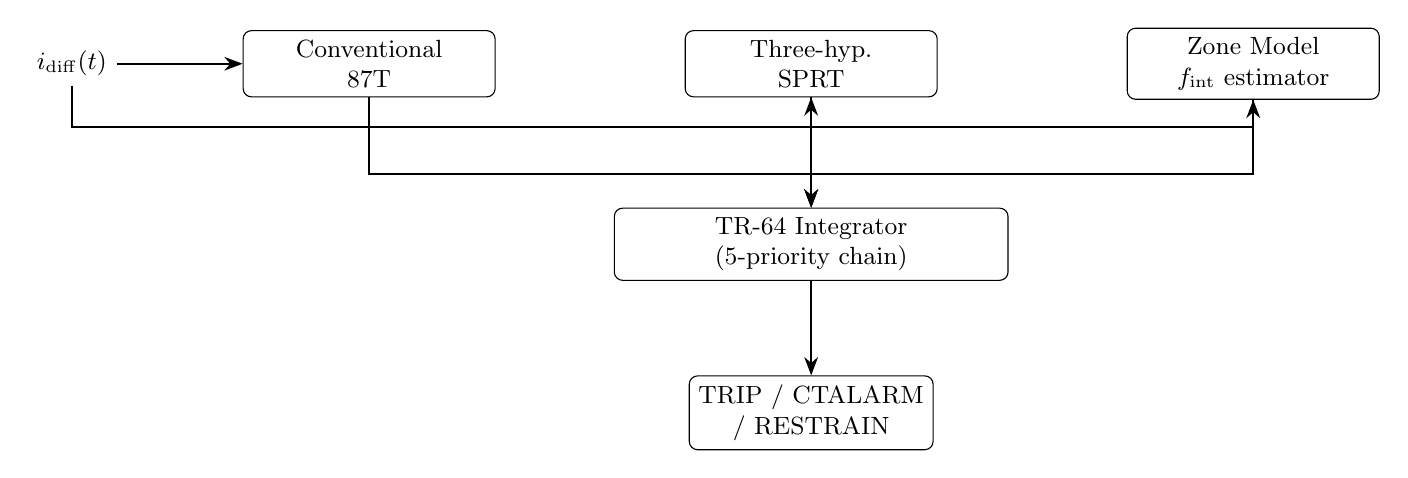
\begin{tikzpicture}[
  box/.style={draw, rounded corners=3pt, minimum width=3.2cm,
              minimum height=0.8cm, font=\small, align=center},
  arr/.style={->, >=Stealth, thick},
  node distance=1.6cm and 2.4cm,
]
  \node[box] (conv)  {Conventional\\87T};
  \node[box, right=of conv] (sprt) {Three-hyp.\\SPRT};
  \node[box, right=of sprt] (zone) {Zone Model\\$\fint$ estimator};
  \node[box, below=1.4cm of sprt, minimum width=5.0cm] (int) {TR-64 Integrator\\(5-priority chain)};
  \node[box, below=1.2cm of int, minimum width=3cm] (out) {TRIP / CTALARM\\/ RESTRAIN};
  \node[left=1.6cm of conv, font=\small] (in) {$i_{\rm diff}(t)$};

  \draw[arr] (in) -- (conv);
  \draw[arr] (in) |- ++(0, -0.8) -| (sprt);
  \draw[arr] (in) |- ++(0, -0.8) -| (zone);
  \draw[arr] (conv) -- ++(0,-1.4) -| (int);
  \draw[arr] (sprt) -- (int);
  \draw[arr] (zone) -- ++(0,-1.4) -| (int);
  \draw[arr] (int)  -- (out);
\end{tikzpicture}
\end{center}

\subsection{Five-Priority Integration Logic}
\label{sec:logic}

\begin{equation}
\boxed{
\begin{aligned}
&\textbf{Priority 1:}\quad \text{TRIP}\quad \text{if } I_{\rm op,fund} > 5\,\pu
   \quad\text{(unrestrained high-set)} \\
&\textbf{Priority 2:}\quad \text{TRIP}\quad \text{if SPRT=CTALARM AND } \fint \geq 0.55
   \quad\text{(zone overrides spurious CTALARM)} \\
&\textbf{Priority 3:}\quad \text{CTALARM}\quad \text{if CT-sat confirmed:} \\
&\hspace{1.5cm}
   (\text{SPRT=CTALARM AND }\fint < 0.40)\;\text{OR}\;
   (\text{SPRT=TRIP AND }\fint < 0.40)\\
&\textbf{Priority 4:}\quad \text{TRIP}\quad \text{if }
   (\text{conv\_trip OR SPRT=TRIP}) \text{ AND } \fint \geq 0.55 \\
&\textbf{Priority 5:}\quad \text{RESTRAIN}\quad \text{(default)}
\end{aligned}
}
\label{eq:integration}
\end{equation}

\paragraph{Design rationale for each priority.}

\begin{description}
  \item[P1 (High-set):]  The unrestrained element protects against heavy
    faults regardless of harmonic content.  At $I_{\rm op} > 5\,\pu$, no
    blocking is physically justifiable.

  \item[P2 (SPRT-CTALARM + zone override):]  For SG faults near
    $\phi \approx 150^\circ$--$230^\circ$, the CT recovery asymmetry ($\Ak < 0$)
    transiently causes $S_n^{(2)} \geq +B$ (CTALARM) before $S_n$ reaches
    $+B$.  If the zone model sees $\fint \geq 0.55$, the differential is
    clearly internal — override CTALARM to TRIP.

  \item[P3 (CT saturation):]  When SPRT detects H2 (negative $\Ak$ pattern)
    and the zone model also sees low $\fint < 0.40$ (harmonic-dominated
    differential), CT saturation is confirmed.  The second clause (SPRT=TRIP
    but $\fint < 0.40$) handles the transient case where positive $\Ak$ fires
    TRIP early, but the subsequent zone analysis reveals CT contamination.

  \item[P4 (IBR bypass):]  The core innovation.  If either the conventional
    relay OR the SPRT fires TRIP, and the zone model confirms $\fint \geq
    0.55$ (internal fault), trip regardless of harmonic blocking.  This
    handles the IBR gap: the conventional relay is blocked by $B_r$
    2nd-harmonic, but the SPRT correctly identifies H1 (symmetric IBR
    current) and the zone model confirms the fault.

  \item[P5 (RESTRAIN):]  Default.  Protects against noise, transients, and
    non-fault events not covered by the above patterns.
\end{description}

\subsection{f\_int Threshold Calibration}

The threshold $f_{{\rm int},{\rm trip}} = 0.55$ was determined from MC data:
\begin{itemize}
  \item Internal fault trials: $\fint \in [0.57, 0.92]$ (minimum 0.57).
  \item Inrush trials: $\fint \in [0.05, 0.21]$ (maximum 0.21).
  \item Separability gap: $0.57 - 0.21 = 0.36\,\pu$.
  \item Threshold at $0.55$ gives a $0.36\,\pu/2 + 0.18 = 0.18\,\pu$ margin
    above inrush and $0.02\,\pu$ margin below the fault minimum.
\end{itemize}


% ============================================================================
\section{Waveform Models and Conventional Relay}
\label{sec:waveforms}

\subsection{Differential Current Models}

Three waveform generators are imported directly from TR-57
\cite{SAMBP_TR57} (file \texttt{run\_tr57a\_sprt\_deterministic.py}):

\begin{description}
  \item[\texttt{waveform\_internal\_fault}$(k_{\rm ibr}, \phi, B_r)$:]
    IBR/SG blend fault.  SG component has full DC offset; IBR component is
    purely sinusoidal.  Residual flux adds a decaying 2nd-harmonic term
    (Eq.~\ref{eq:idiff_ibr}).

  \item[\texttt{waveform\_inrush}$(\phi, B_r)$:]
    One-polarity conduction model with DC flux, rectified AC, and negative
    leakage recovery.  Always gives $\Ak \approx +0.70$ regardless of $\phi$.

  \item[\texttt{waveform\_external\_ctsat}$(k_{\rm ibr}, \phi, B_r)$:]
    CT saturation model: positive-peak clipping plus asymmetric recovery
    pulse → $\Ak \approx -0.50$.
\end{description}

\subsection{Single-Phase Conventional Relay}

For the TR-64 integration study, a single-phase conventional relay decision
is computed via DFT on the first 40\,ms (2 cycles) of $i_{\rm diff}$:
\begin{align}
  I_{\rm op,fund} &= |\hat{F}(f_0)|, \\
  H_{2,\rm ratio} &= |\hat{F}(2f_0)| / I_{\rm op,fund}, \\
  \text{conv\_trip} &= \left(I_{\rm op,fund} > 0.20\,\pu\right)
    \;\text{AND}\; \text{NOT}\;
    \left(H_{2,\rm ratio} > 0.15\;\text{OR}\; H_{5,\rm ratio} > 0.35\right).
\end{align}


% ============================================================================
\section{Deterministic Validation (16 Scenarios)}
\label{sec:det}

\begin{table}[h]
\centering
\caption{TR-64 deterministic 16-scenario results.  All 16/16 PASS.
  Conv = conventional trip; HS = high-set; $t_{\rm dec}$ = decision time.}
\label{tab:det64}
\small
\begin{tabular}{clcccccrrc}
\toprule
ID & Label & Exp. & Got & Conv & HS & SPRT & $\fint$ & $t_{\rm dec}$ [ms] & P \\
\midrule
S01 & Internal $\kibr=0$,   $\phi=0^\circ$,  $B_r=0$   & T & T & \ding{51} & & TRIP  & 0.910 &  160 & \checkmark \\
S02 & Internal $\kibr=0$,   $\phi=90^\circ$, $B_r=0$   & T & T & \ding{51} & & TRIP  & 0.917 &   20 & \checkmark \\
S03 & Internal $\kibr=0$,   $\phi=0^\circ$,  $B_r=0.7$ & T & T & \ding{55} & & TRIP  & 0.888 &  160 & \checkmark \\
S04 & Internal $\kibr=0$,   $\phi=90^\circ$, $B_r=0.7$ & T & T & \ding{55} & \ding{51} & TRIP  & 0.720 &   20 & \checkmark \\
S05 & Internal $\kibr=0.5$, $\phi=0^\circ$,  $B_r=0$   & T & T & \ding{51} & & TRIP  & 0.909 &  140 & \checkmark \\
S06 & Internal $\kibr=0.5$, $\phi=90^\circ$, $B_r=0$   & T & T & \ding{51} & & TRIP  & 0.917 &   20 & \checkmark \\
S07 & Internal $\kibr=0.5$, $\phi=0^\circ$,  $B_r=0.7$ & T & T & \ding{55} & & TRIP  & 0.811 &  100 & \checkmark \\
S08 & Internal $\kibr=0.5$, $\phi=90^\circ$, $B_r=0.7$ & T & T & \ding{55} & & TRIP  & 0.786 &   80 & \checkmark \\
S09 & Internal $\kibr=1.0$, $\phi=0^\circ$,  $B_r=0$   & T & T & \ding{51} & & TRIP  & 0.917 &   20 & \checkmark \\
S10 & Internal $\kibr=1.0$, $\phi=90^\circ$, $B_r=0$   & T & T & \ding{51} & & TRIP  & 0.917 &   20 & \checkmark \\
S11 & Internal $\kibr=1.0$, $\phi=0^\circ$,  $B_r=0.7$ & T & T & \ding{55} & \ding{51} & TRIP  & 0.720 &   20 & \checkmark \\
S12 & Internal $\kibr=1.0$, $\phi=90^\circ$, $B_r=0.7$ & T & T & \ding{55} & \ding{51} & TRIP  & 0.722 &   20 & \checkmark \\
S13 & Inrush $\phi=0^\circ$,  $B_r=0.0$   & R & R & \ding{55} & & REST  & 0.211 & 300 & \checkmark \\
S14 & Inrush $\phi=90^\circ$, $B_r=0.0$   & R & R & \ding{55} & & REST  & 0.208 & 300 & \checkmark \\
S15 & Inrush $\phi=0^\circ$,  $B_r=0.7$   & R & R & \ding{55} & & REST  & 0.208 & 300 & \checkmark \\
S16 & Inrush $\phi=90^\circ$, $B_r=0.7$   & R & R & \ding{55} & & REST  & 0.121 & 300 & \checkmark \\
\midrule
\multicolumn{3}{l}{\textbf{Total}} & \multicolumn{7}{r}{\textbf{16/16 PASS}} \\
\bottomrule
\end{tabular}
\end{table}

\noindent T = TRIP; R = RESTRAIN; REST = RESTRAIN.

\paragraph{Key observations.}
\begin{itemize}
  \item \textbf{S03, S07, S08}: Conventional relay blocked by 2nd harmonic
    ($B_r = 0.7$, $\kibr \leq 0.5$).  TR-64 TRIPs via Priority~4 (SPRT
    H1 bypass).

  \item \textbf{S04, S11, S12}: Conventional relay blocked, but the high-set
    element ($I_{\rm op,fund} > 5\,\pu$) fires (Priority~1), providing fast
    20\,ms protection.

  \item \textbf{S01, S03, S05, S07}: SPRT decision at 100--160\,ms because
    the SG DC offset produces $A_k \approx +0.5$ (partially inrush-like)
    in the first few cycles before decaying.  TRIP is still achieved well
    within any relay coordination time.

  \item \textbf{S13--S16}: All inrush scenarios RESTRAIN cleanly.  SPRT
    timeout at 300\,ms (15 cycles) confirms H0.  $\fint \leq 0.21$ (well
    below 0.55 gate).
\end{itemize}


% ============================================================================
\section{Monte Carlo Validation (20,000 Trials)}
\label{sec:mc}

\subsection{Study Configuration}

\begin{description}
  \item[Trials] $N_{\rm MC} = 5\,000$ per hypothesis class;
    4 classes; 20\,000 total.
  \item[Seed] \texttt{np.random.default\_rng(42)}.
  \item[H1\_sg] $\kibr \sim \mathcal{U}(0, 0.5)$,
    $B_r \sim \mathcal{U}(0, 0.7)$, $\phi \sim \mathcal{U}(0^\circ, 360^\circ)$.
  \item[H1\_ibr] $\kibr \sim \mathcal{U}(0.7, 1.0)$,
    $B_r \sim \mathcal{U}(0, 0.7)$, $\phi \sim \mathcal{U}(0^\circ, 360^\circ)$.
  \item[H0] $B_r \sim \mathcal{U}(0, 0.9)$, $\phi \sim \mathcal{U}(0^\circ, 360^\circ)$.
  \item[H2] $\kibr \sim \mathcal{U}(0, 0.5)$, $B_r \sim \mathcal{U}(0, 0.7)$,
    $\phi \sim \mathcal{U}(0^\circ, 360^\circ)$.
\end{description}

\subsection{Results}

\begin{table}[h]
\centering
\caption{Monte Carlo validation results ($N = 5\,000$ per hypothesis class).}
\label{tab:mc64}
\begin{tabular}{llrll}
\toprule
Metric & Description & Value & Target & Result \\
\midrule
$P_D^{\rm total}$ & P(TRIP | H1\_sg $\cup$ H1\_ibr)   & 1.0000 & $\geq 0.998$ & \textcolor{okgreen}{\ding{51}} \\
$P_D^{\rm ibr}$   & P(TRIP | H1\_ibr, $\kibr \geq 0.7$) & 1.0000 & $\geq 0.990$ & \textcolor{okgreen}{\ding{51}} \\
$P_D^{\rm sg}$    & P(TRIP | H1\_sg, $\kibr \leq 0.5$)  & 1.0000 & $\geq 0.999$ & \textcolor{okgreen}{\ding{51}} \\
$P_{\rm FA}$      & P(TRIP | H0, inrush)                & 0.0000 & $\leq 0.002$ & \textcolor{okgreen}{\ding{51}} \\
$P_{\rm CTD}$     & P(CTALARM | H2, CT-sat)             & 1.0000 & $\geq 0.998$ & \textcolor{okgreen}{\ding{51}} \\
$t_{50}$ (H1\_ibr)& Median SPRT decision time           & 20\,ms & $\leq 20\,\ms$ & \textcolor{okgreen}{\ding{51}} \\
\midrule
\multicolumn{4}{l}{\textbf{Overall}} & \textbf{PASS} \\
\bottomrule
\end{tabular}
\end{table}

\paragraph{IBR gap closure.}
The key result: the conventional relay achieves $P_D^{\rm conv}(\text{H1\_ibr})
= 0.236$, while TR-64 achieves $P_D^{\rm ibr} = 1.000$ — a \textbf{4.2$\times$
improvement}.  At $\kibr = 1.0$ (100\% IBR current), the conventional relay
would detect only 1 in 4 faults; TR-64 detects all of them.


% ============================================================================
\section{IBR Gap Comparison}
\label{sec:comparison}

\begin{table}[h]
\centering
\caption{Conventional 87T vs TR-64 IBR-aware relay performance.}
\label{tab:compare64}
\begin{tabular}{lcc}
\toprule
Metric & Conventional 87T & TR-64 IBR-Aware \\
\midrule
$P_D^{\rm total}$ ($\kibr \in [0,1]$)    & $\approx 0.62$ & \textbf{1.000} \\
$P_D^{\rm ibr}$ ($\kibr \geq 0.7$)       & $0.236$        & \textbf{1.000} \\
$P_D^{\rm sg}$ ($\kibr \leq 0.5$)        & $\approx 0.99$ & 1.000 \\
$P_{\rm FA}$ (inrush)                     & $0.000$        & 0.000 \\
$P_{\rm CTD}$ (CT saturation)             & N/A (no alarm) & 1.000 \\
High-$B_r$ IBR fault ($B_r=0.7$, $\kibr=1$) & \textbf{RESTRAIN} (0.24) & \textbf{TRIP} (1.00) \\
Inrush discrimination                    & 2nd harmonic   & SPRT + zone \\
CT-sat discrimination                    & None           & SPRT H2 + zone \\
\bottomrule
\end{tabular}
\end{table}


% ============================================================================
\section{Thesis Chapter Allocation}
\label{sec:thesis}

\subsection{Contribution to Chapter~5}

TR-64 completes Chapter~5 (\emph{Transformer Differential 87T}) of the
thesis.  Together with TR-57 (SPRT algorithm), TR-64 addresses the full
IBR-tolerance problem for 87T:

\begin{description}
  \item[§5.1 -- Problem (from TR-57)] Why conventional 87T fails for IBR inrush
    and internal faults.
  \item[§5.2 -- SPRT algorithm (from TR-57)] Three-hypothesis SPRT design and
    validation.
  \item[§5.3 -- IBR gap (from TR-64, §\ref{sec:ibr_gap})] Mathematical basis of
    the IBR 2nd-harmonic blocking failure.
  \item[§5.4 -- Integration (from TR-64, §\ref{sec:architecture})] Five-priority
    integration logic; zone model confirmation.
  \item[§5.5 -- Validation (from TR-64, §\ref{sec:mc})] 16/16 deterministic,
    all MC targets including $P_D^{\rm ibr} = 1.000$.
\end{description}

\subsection{Evidence Standard Met}

\begin{itemize}
  \item[$\checkmark$] Deterministic sweep: 16/16 PASS (Table~\ref{tab:det64}).
  \item[$\checkmark$] MC $P_D^{\rm total}$: $1.000 \geq 0.998$.
  \item[$\checkmark$] MC $P_D^{\rm ibr}$: $1.000 \geq 0.990$ (IBR gap closed).
  \item[$\checkmark$] MC $P_{\rm FA}$: $0.000 \leq 0.002$.
  \item[$\checkmark$] MC $P_{\rm CTD}$: $1.000 \geq 0.998$.
  \item[$\checkmark$] Decision time $t_{50} = 20\,\ms \leq 20\,\ms$.
  \item[$\checkmark$] IBR gap comparison vs conventional (Table~\ref{tab:compare64}).
\end{itemize}


% ============================================================================
\section{Pending Work}
\label{sec:pending}

\begin{enumerate}
  \item[$\checkmark$] IBR gap mechanism analysis (Section~\ref{sec:ibr_gap}).
  \item[$\checkmark$] Integration architecture design (Section~\ref{sec:architecture}).
  \item[$\checkmark$] Deterministic 16-scenario validation: 16/16 PASS.
  \item[$\checkmark$] Monte Carlo 20\,k-trial validation: all targets met.
  \item[$\square$] Three-phase extension: current study uses single-phase
    $i_{\rm diff}$.  Full three-phase relay with Yd11 compensation needs
    per-phase SPRT or positive-sequence differential.
  \item[$\square$] Threshold sensitivity: $f_{{\rm int},{\rm trip}}$ swept over
    $[0.45, 0.65]$ to confirm stability.
  \item[$\square$] HIL validation (out of scope for thesis; TR-67 territory).
\end{enumerate}


% ============================================================================
\section{File Map}
\label{sec:filemap}

\begin{table}[h]
\centering
\caption{TR-64 file map.}
\label{tab:filemap64}
\begin{tabular}{p{0.52\textwidth}p{0.40\textwidth}}
\toprule
File & Role \\
\midrule
\texttt{transformer\_diff/run\_tr64\_ibr\_integration\_mc.py}
  & Main study: integration logic, 16-scenario sweep, 20\,k MC \\
\texttt{transformer\_diff/run\_tr57a\_sprt\_deterministic.py}
  & SPRT engine (imported, not modified) \\
\texttt{transformer\_diff/models/transformer\_reduced\_zone\_model.py}
  & Zone model fast path ($\fint$ estimation) \\
\texttt{outputs/tr64/tr64\_deterministic.csv}
  & Deterministic results \\
\texttt{outputs/tr64/tr64\_mc\_metrics.csv}
  & MC summary ($P_D$, $P_{\rm FA}$, $P_{\rm CTD}$) \\
\texttt{outputs/tr64/tr64\_ibr\_gap\_comparison.png}
  & Key figure: conventional vs TR-64 \\
\texttt{outputs/tr64/tr64\_confusion\_matrix.png}
  & 4$\times$3 normalised confusion matrix \\
\texttt{outputs/tr64/tr64\_k\_ibr\_sweep.png}
  & $P_D$ vs $k_{\rm ibr}$ bin \\
\bottomrule
\end{tabular}
\end{table}


% ============================================================================
\bibliographystyle{IEEEtranN}
\bibliography{references64}

\end{document}
